%%This is a standard LaTeX2e article document template. personal version 12/5/200%%
\documentclass[11pt,twoside]{article}
%%%%%%%%%%%%%%%%%%%%%%%%%%%%%%%packages%%%%%%%%%%%%%%%%%%%%%%%%%%%%%%%%%%%%%%%%%%%%%%%%%%%%%%%%%%
\pagestyle{empty}

\usepackage{latexsym}
\usepackage{amssymb}
\usepackage{amsfonts}
\usepackage{amstext}
\usepackage{amsmath, amsthm}
\usepackage{multicol}
\usepackage{hyperref}
\usepackage{graphicx}
\usepackage{tikz}
\usepackage{wrapfig}
\usepackage{enumitem}
\usepackage{float}
\usepackage{caption}
\usepackage{hyperref}
\hypersetup{
    colorlinks=true,
    linkcolor=blue,
    filecolor=magenta,      
    urlcolor=cyan
    }

%%%%%%%%%%%%%%%%%%%%%%%%%%%%%%%formatting%%%%%%%%%%%%%%%%%%%%%%%%%%%%%%%%%%%%%%%%%%%%%%%%%%%%%%%
\setlength{\topmargin}{0in}        %%%  This sets all the spacing stuff to use the page more
\setlength{\oddsidemargin}{0in}    %%%  efficiently than the normal "article" setup would.
\setlength{\evensidemargin}{0in}   %%%  It's OK to play with these some.
\setlength{\textheight}{9in}     %%%
\setlength{\textwidth}{6.25in}     %%%
\setlength{\headsep}{0in}          %%%
\setlength{\headheight}{0in}       %%%
%\setlength{\footskip}{0in}         %%%
\linespread{1.25}

%%%%%%%%%%%%%%%%%%%%%%%%%%%%%%%%%%%%%%%%%%%%%%%%%%%%%%%%%%%%%%%%%%%%%%%%%%%%%%%%%%%%%%%%%%%%%%%

\begin{document}

\begin{center}
{\bf \Large Math 335, Topic \#2 Final Project}\\
\vspace{0.1in}
{\Large Due Wednesday, May 12}\\
\vspace{0.1cm}
{\large Mark Kim}
\end{center}

\hrule

\vspace{.2in}

Topic 2 is an exploration of the \emph{Orbit-Stabilizer Theorem} and \emph{Symmetries}.  Lagrange's Theorem and the Orbit-Stabilizer Theorem are both counting theorems which enable us to find the quantity of elements in different sets, the latter of which allows us to find the number of elements in any finite group of permutations of a set.  In fact, Lagrange's Theorem provides us with a method for proving the Orbit-Stabilizer Theorem.  Armed with an understanding of the Orbit-Stabilizer Theorem, we find that it can accurately count the number of symmetries of different polyhedra.  Specifically, we explored the cube, tetrahedron, octahedron, dodecahedron, and truncated icosehedron.  In this paper, I will discuss the Orbit-Stabilizer Theorem, and how it relates to our understanding of cosets and symmetries of the aforementioned polyhedra.

To understand this subject, we must establish some definitions upon which the Orbit-Stabilizer Theorem is built.  Let us first define the \emph{permutation} and \emph{permutation group}.  As defined in Gallian's \emph{Contemporary Abstract Algebra},
\begin{quote}
A \emph{permutation} of a set $A$ is a function from $A$ to $A$ that is both one-to-one and onto.  A \emph{permutation group} of a set $A$ is a set of permutations of $A$ that forms a group under function composition. (93)
\end{quote}
To give an example of a permutation group, consider the set of faces of a cube,
\[ A = \{ \text{faces of a cube} \}. \]
I interpret this set $A$ as the infinite set of functions that take a face of a cube and ``moves'' it to a particular location or orientation.  Then a permutation group of $A$ could be
\[ C = \{ \text{rotational symmetries of a cube} \}. \]
This group $C$ are all the functions in $A$ that maintain rotational symmetries of the cube.  So if we pick a single function $a\in A$ that produces a particular location and orientation, $C$ contains the functions that will produce all rotational symmetries from that particular $a$.\footnote{I am having a little bit of a hard time conceptualizing these terms and producing an example from it.  I hope my explanation is not too confusing or misleading.}

From our established understanding of the a permutation group, the \emph{stabilizer of a point} can be defined:
%%%%%%%%%%%%%%%%%%%%%%%%%%%%%%%%%%
% STABILIZER
%%%%%%%%%%%%%%%%%%%%%%%%%%%%%%%%%%
\begin{quote}
Let $G$ be a group of permutations of a set $S$.  For each $i$ in $S$, let $\operatorname{stab}_G(i) = \{ \phi \in G\, | \, \phi(i) = i \}$.  We call $\operatorname{stab}_G(i)$ the \emph{stabilizer} of $i$ in $G$. (Gallian 152)
\end{quote}
What this first definition describes is the set of elements in $G$ which leave $i$ fixed. To illustrate this, let us revisit the cube with 6 faces described earlier and the permutation group $C$. Let $f$ be a single fixed face of the cube.  The stabilizer of $f$ in $C$ is the set of facings possible while maintaining symmetry.  In this case, there are 4 different possible facings of the cube as shown in Figure \ref{stab}.

\begin{figure}[H]\centering
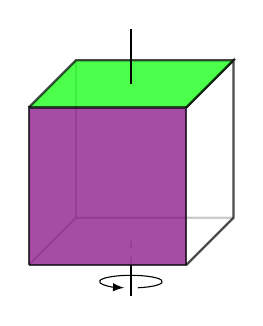
\begin{tikzpicture}[thick,scale=2]
    \coordinate (A1) at (0, 0);
    \coordinate (A2) at (0, 1);
    \coordinate (A3) at (1, 1);
    \coordinate (A4) at (1, 0);
    \coordinate (B1) at (0.3, 0.3);
    \coordinate (B2) at (0.3, 1.3);
    \coordinate (B3) at (1.3, 1.3);
    \coordinate (B4) at (1.3, 0.3);
    \coordinate (R1) at (0.65, 1.5);
    \coordinate (R2) at (0.65, 1.15);
    \coordinate (R3) at (0.65, 0);
    \coordinate (R4) at (0.65, -0.2);
    \coordinate (R5) at (0.65, 0.15);
	\draw[dashed, opacity=0.2] (R3) -- (R5);

%	\node[xscale=-1, opacity=0.4, scale=1.5] at (0.8,0.8) {4};
%	\node[style={yslant=.6},yslant=.6,xscale=-.5, yscale=1, scale=1.5, opacity=0.4] at (0.15,0.65) {5};
%	\node[style={yslant=.05, xslant=.6},yslant=0.05, xslant=.6, yscale=-0.5, scale=1.5, opacity=0.4] at (0.65,0.15) {6};

    \draw[opacity=0.2] (A1) -- (B1) -- (B4);
    \draw[opacity=0.2] (B2) -- (B1);
    % \draw[opacity=0.2] (B1) -- (B2) -- (B3) -- (B4);
    \draw[opacity=0.7] (A3) -- (B3) -- (B4) -- (A4);
    \draw[fill=green,opacity=0.7] (A2) -- (B2) -- (B3) -- (A3);
    \draw[fill=violet,opacity=0.7] (A1) -- (A2) -- (A3) -- (A4) -- (A1);

	\draw[solid] (R1) -- (R2);
	\draw[solid] (R3) -- (R4);
    \draw[thin, -latex, xshift=18.5, yshift=-3] (-77.5:2mm and 0.4mm) arc (-77:257.5:2mm and 0.4mm);
    
%	\node[style={yslant=.05, xslant=.6},yslant=0.05, xslant=.6, scale=1.5, yscale=0.5] at (0.65,1.15) {1};
%	\node[scale=1.5] at (0.5,0.5) {2};
%	\node[style={yslant=.6},yslant=.6, xscale=0.5, scale=1.5, yscale=1] at (01.15, 0.65) {3};
\end{tikzpicture}\quad
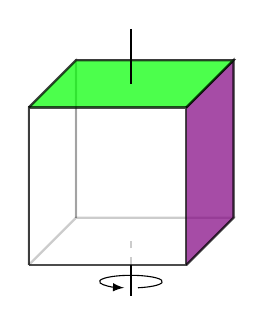
\begin{tikzpicture}[thick,scale=2]
    \coordinate (A1) at (0, 0);
    \coordinate (A2) at (0, 1);
    \coordinate (A3) at (1, 1);
    \coordinate (A4) at (1, 0);
    \coordinate (B1) at (0.3, 0.3);
    \coordinate (B2) at (0.3, 1.3);
    \coordinate (B3) at (1.3, 1.3);
    \coordinate (B4) at (1.3, 0.3);
    \coordinate (R1) at (0.65, 1.5);
    \coordinate (R2) at (0.65, 1.15);
    \coordinate (R3) at (0.65, 0);
    \coordinate (R4) at (0.65, -0.2);
    \coordinate (R5) at (0.65, 0.15);
	\draw[dashed, opacity=0.2] (R3) -- (R5);

%1 green
%2 violet
%3 red
%4 orange
%5 yellow
%6 pink

%	\node[xscale=-1, opacity=0.4, scale=1.5] at (0.8,0.8) {3}; 
%	\node[style={yslant=.6},yslant=.6,xscale=-.5, yscale=1, opacity=0.4, scale=1.5] at (0.15,0.65) {4}; 
%	\node[style={xslant=.6},xslant=.6, yscale=-0.5, rotate=-90, opacity=0.4, scale=1.5] at (0.65,0.15) {6};

    \draw[opacity=0.2] (A1) -- (B1) -- (B4) -- (A4); % bottom
    \draw[opacity=0.2] (A1) -- (A2) -- (B2) -- (B1); % left
    \draw[opacity=0.2] (B1) -- (B2) -- (B3) -- (B4); % back
    \draw[fill=violet,opacity=0.7] (A3) -- (B3) -- (B4) -- (A4); % right
    \draw[fill=green,opacity=0.7] (A2) -- (B2) -- (B3) -- (A3); % top
    \draw[opacity=0.7] (A1) -- (A2) -- (A3) -- (A4) -- (A1) -- (A1); % front

	\draw[solid] (R1) -- (R2);
	\draw[solid] (R3) -- (R4);
    \draw[thin, -latex, xshift=18.5, yshift=-3] (-77.5:2mm and 0.4mm) arc (-77:257.5:2mm and 0.4mm);
    
%		\node[style={xslant=.6},xslant=.6, yscale=0.5, rotate=90, scale=1.5] at (0.65,1.15) {1}; % green
%		\node[scale=1.5] at (0.5,0.5) {5}; % violet
%		\node[style={yslant=.6},yslant=.6, xscale=0.5, yscale=1, scale=1.5] at (01.15, 0.65) {2}; % red
\end{tikzpicture}\quad
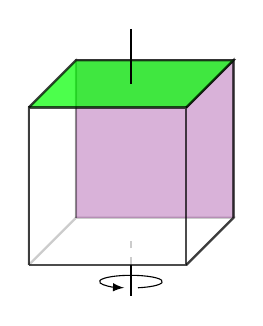
\begin{tikzpicture}[thick,scale=2]
    \coordinate (A1) at (0, 0);
    \coordinate (A2) at (0, 1);
    \coordinate (A3) at (1, 1);
    \coordinate (A4) at (1, 0);
    \coordinate (B1) at (0.3, 0.3);
    \coordinate (B2) at (0.3, 1.3);
    \coordinate (B3) at (1.3, 1.3);
    \coordinate (B4) at (1.3, 0.3);
    \coordinate (R1) at (0.65, 1.5);
    \coordinate (R2) at (0.65, 1.15);
    \coordinate (R3) at (0.65, 0);
    \coordinate (R4) at (0.65, -0.2);
    \coordinate (R5) at (0.65, 0.15);
	\draw[dashed, opacity=0.2] (R3) -- (R5);

%1 green
%2 violet
%3 red
%4 orange
%5 yellow
%6 pink
%
%	\node[xscale=-1, opacity=0.4, scale=1.5] at (0.8,0.8) {2}; 
%	\node[style={yslant=.6},yslant=.6,xscale=-.5, yscale=1, opacity=0.4, scale=1.5] at (0.15,0.65) {3}; 
%	\node[style={xslant=.6},xslant=.6, yscale=-0.5, rotate=180, opacity=0.4, scale=1.5] at (0.65,0.15) {6};

    \draw[opacity=0.2] (A1) -- (B1) -- (B4) -- (A4); % bottom
    \draw[opacity=0.2] (A1) -- (A2) -- (B2) -- (B1); % left
    \draw[fill=violet,opacity=0.3] (B1) -- (B2) -- (B3) -- (B4); % back
    \draw[opacity=0.7] (A3) -- (B3) -- (B4) -- (A4); % right
    \draw[fill=green,opacity=0.7] (A2) -- (B2) -- (B3) -- (A3); % top
    \draw[opacity=0.7] (A1) -- (A2) -- (A3) -- (A4) -- (A1); % front

	\draw[solid] (R1) -- (R2);
	\draw[solid] (R3) -- (R4);
    \draw[thin, -latex, xshift=18.5, yshift=-3] (-77.5:2mm and 0.4mm) arc (-77:257.5:2mm and 0.4mm);
    
%	\node[style={xslant=.6},xslant=.6, yscale=0.5, rotate=-180, scale=1.5] at (0.65,1.15) {1}; % green
%	\node[scale=1.5] at (0.5,0.5) {4}; % violet
%	\node[style={yslant=.6},yslant=.6, xscale=0.5, yscale=1, scale=1.5] at (01.15, 0.65) {5}; % red
\end{tikzpicture}\quad
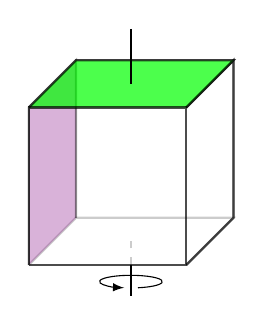
\begin{tikzpicture}[thick,scale=2]
    \coordinate (A1) at (0, 0);
    \coordinate (A2) at (0, 1);
    \coordinate (A3) at (1, 1);
    \coordinate (A4) at (1, 0);
    \coordinate (B1) at (0.3, 0.3);
    \coordinate (B2) at (0.3, 1.3);
    \coordinate (B3) at (1.3, 1.3);
    \coordinate (B4) at (1.3, 0.3);
    \coordinate (R1) at (0.65, 1.5);
    \coordinate (R2) at (0.65, 1.15);
    \coordinate (R3) at (0.65, 0);
    \coordinate (R4) at (0.65, -0.2);
    \coordinate (R5) at (0.65, 0.15);
	\draw[dashed, opacity=0.2] (R3) -- (R5);

%1 green
%2 violet
%3 red
%4 orange
%5 yellow
%6 pink

%	\node[xscale=-1, opacity=0.4, scale=1.5] at (0.8,0.8) {5}; 
%	\node[style={yslant=.6},yslant=.6,xscale=-.5, yscale=1, opacity=0.4, scale=1.5] at (0.15,0.65) {2}; 
%	\node[style={xslant=.6},xslant=.6, yscale=-0.5, rotate=90, opacity=0.4, scale=1.5] at (0.65,0.15) {6};

    \draw[opacity=0.2] (A1) -- (B1) -- (B4) -- (A4); % bottom
    \draw[fill=violet,opacity=0.3] (A1) -- (A2) -- (B2) -- (B1); % left
    \draw[opacity=0.2] (B1) -- (B2) -- (B3) -- (B4); % back
    \draw[opacity=0.7] (A3) -- (B3) -- (B4) -- (A4); % right
    \draw[fill=green,opacity=0.7] (A2) -- (B2) -- (B3) -- (A3); % top
    \draw[opacity=0.7] (A1) -- (A2) -- (A3) -- (A4) -- (A1); % front

	\draw[solid] (R1) -- (R2);
	\draw[solid] (R3) -- (R4);
    \draw[thin, -latex, xshift=18.5, yshift=-3] (-77.5:2mm and 0.4mm) arc (-77:257.5:2mm and 0.4mm);
    
%	\node[style={xslant=.6},xslant=.6, yscale=0.5, rotate=-90, scale=1.5] at (0.65,1.15) {1}; % green
%	\node[scale=1.5] at (0.5,0.5) {3}; % violet
%	\node[style={yslant=.6},yslant=.6, xscale=0.5, yscale=1, scale=1.5] at (01.15, 0.65) {4}; % red
\end{tikzpicture}
\caption{4 possible facings of a cube with side 1 fixed in place ($|\operatorname{stab}_{C}(f)| = 4$)}
\label{stab}
\end{figure}
Following a similar convention to the cube, we can find the number of elements for a particular face of a tetrahedron, where
\[ T = \{ \text{rotational symmetries of a tetrahedron} \}. \]
Fixing the bottom face, a symmetry can be found by composing 120 degree rotations, giving us $\operatorname{stab}_{T}(f) = \{ I, R_{120}, R_{240} \}$ and $|\operatorname{stab}_{T}(f)| = 3$.

%%%%%%%%%%
% ORBIT
%%%%%%%%%%
The next term we will examine is the \emph{orbit of a point}:
\begin{quote}
Let $G$ be a group of permutations of a set $S$.  For each $s$ in $S$, let $\operatorname{orb}_G(s) = \{ \phi(s)\, | \, \phi \in G \}$.  The set $\operatorname{orb}_G(s)$ is a subset of $S$ called the \emph{orbit of s under} $G$. (Gallian 152)
\end{quote}
This definition categorizes all the elements of the set $S$ towards which a particular element can be sent to by group $G$.  Using our previous example of a cube, the orbit of a face under $C$ is the set of possible locations that the face can be carried to within $S$ by $C$.  In other words, it is the set of locations that the face can occupy while maintaining symmetry.  This is illustrated in Figure \ref{orb}.  Likewise, the same can be found for a tetrahedron, resulting in $|\operatorname{orb}_{T}(f)| = 4$.
\begin{figure}[H]\centering
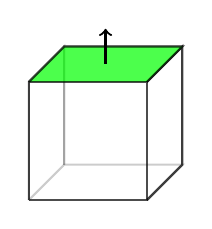
\begin{tikzpicture}[thick,scale=1.5]
    \coordinate (A1) at (0, 0);
    \coordinate (A2) at (0, 1);
    \coordinate (A3) at (1, 1);
    \coordinate (A4) at (1, 0);
    \coordinate (B1) at (0.3, 0.3);
    \coordinate (B2) at (0.3, 1.3);
    \coordinate (B3) at (1.3, 1.3);
    \coordinate (B4) at (1.3, 0.3);
    \coordinate (R1) at (0.65, 1.45);
    \coordinate (R2) at (0.65, 1.15);
	
%1 green
%2 violet
%3 red
%4 orange
%5 yellow
%6 pink

    \draw[opacity=0.2] (A1) -- (B1) -- (B4) -- (A4); % bottom
    \draw[opacity=0.2] (A1) -- (A2) -- (B2) -- (B1); % left
    \draw[opacity=0.2] (B1) -- (B2) -- (B3) -- (B4); % back
    \draw[opacity=0.7] (A3) -- (B3) -- (B4) -- (A4); % right
    \draw[fill=green,opacity=0.7] (A2) -- (B2) -- (B3) -- (A3); % top
    \draw[opacity=0.7] (A1) -- (A2) -- (A3) -- (A4) -- (A1) -- (A1); % front
    
	\draw[<-] (R1) -- (R2);
    
\end{tikzpicture}\quad
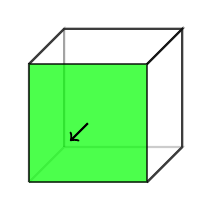
\begin{tikzpicture}[thick,scale=1.5]
    \coordinate (A1) at (0, 0);
    \coordinate (A2) at (0, 1);
    \coordinate (A3) at (1, 1);
    \coordinate (A4) at (1, 0);
    \coordinate (B1) at (0.3, 0.3);
    \coordinate (B2) at (0.3, 1.3);
    \coordinate (B3) at (1.3, 1.3);
    \coordinate (B4) at (1.3, 0.3);
    \coordinate (R1) at (0.35, 0.35);
    \coordinate (R2) at (0.5, 0.5);
	
%1 green
%2 violet
%3 red
%4 orange
%5 yellow
%6 pink

    \draw[opacity=0.2] (A1) -- (B1) -- (B4) -- (A4); % bottom
    \draw[opacity=0.2] (A1) -- (A2) -- (B2) -- (B1); % left
    \draw[opacity=0.2] (B1) -- (B2) -- (B3) -- (B4); % back
    \draw[opacity=0.7] (A3) -- (B3) -- (B4) -- (A4); % right
    \draw[opacity=0.7] (A2) -- (B2) -- (B3) -- (A3); % top
    \draw[fill=green,opacity=0.7] (A1) -- (A2) -- (A3) -- (A4) -- (A1) -- (A1); % front
    
	\draw[<-] (R1) -- (R2);
    
\end{tikzpicture}\quad
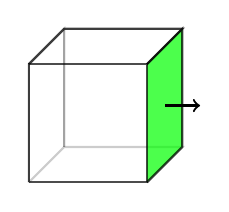
\begin{tikzpicture}[thick,scale=1.5]
    \coordinate (A1) at (0, 0);
    \coordinate (A2) at (0, 1);
    \coordinate (A3) at (1, 1);
    \coordinate (A4) at (1, 0);
    \coordinate (B1) at (0.3, 0.3);
    \coordinate (B2) at (0.3, 1.3);
    \coordinate (B3) at (1.3, 1.3);
    \coordinate (B4) at (1.3, 0.3);
    \coordinate (R1) at (1.45, 0.65);
    \coordinate (R2) at (1.15, 0.65);
	
%1 green
%2 violet
%3 red
%4 orange
%5 yellow
%6 pink

    \draw[opacity=0.2] (A1) -- (B1) -- (B4) -- (A4); % bottom
    \draw[opacity=0.2] (A1) -- (A2) -- (B2) -- (B1); % left
    \draw[opacity=0.2] (B1) -- (B2) -- (B3) -- (B4); % back
    \draw[fill=green, opacity=0.7] (A3) -- (B3) -- (B4) -- (A4); % right
    \draw[opacity=0.7] (A2) -- (B2) -- (B3) -- (A3); % top
    \draw[opacity=0.7] (A1) -- (A2) -- (A3) -- (A4) -- (A1) -- (A1); % front
    
	\draw[<-] (R1) -- (R2);
    
\end{tikzpicture}\quad
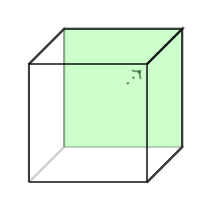
\begin{tikzpicture}[thick,scale=1.5]
    \coordinate (A1) at (0, 0);
    \coordinate (A2) at (0, 1);
    \coordinate (A3) at (1, 1);
    \coordinate (A4) at (1, 0);
    \coordinate (B1) at (0.3, 0.3);
    \coordinate (B2) at (0.3, 1.3);
    \coordinate (B3) at (1.3, 1.3);
    \coordinate (B4) at (1.3, 0.3);
    \coordinate (R1) at (0.95, 0.95);
    \coordinate (R2) at (0.8, 0.8);

	\draw[dotted, <-, opacity=0.5] (R1) -- (R2);
	
%1 green
%2 violet
%3 red
%4 orange
%5 yellow
%6 pink

    \draw[opacity=0.2] (A1) -- (B1) -- (B4) -- (A4); % bottom
    \draw[opacity=0.2] (A1) -- (A2) -- (B2) -- (B1); % left
    \draw[fill=green, opacity=0.2] (B1) -- (B2) -- (B3) -- (B4); % back
    \draw[opacity=0.7] (A3) -- (B3) -- (B4) -- (A4); % right
    \draw[opacity=0.7] (A2) -- (B2) -- (B3) -- (A3); % top
    \draw[opacity=0.7] (A1) -- (A2) -- (A3) -- (A4) -- (A1) -- (A1); % front
    
\end{tikzpicture}\quad
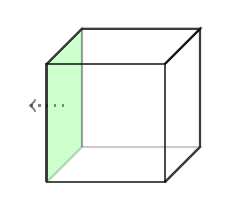
\begin{tikzpicture}[thick,scale=1.5]
    \coordinate (A1) at (0, 0);
    \coordinate (A2) at (0, 1);
    \coordinate (A3) at (1, 1);
    \coordinate (A4) at (1, 0);
    \coordinate (B1) at (0.3, 0.3);
    \coordinate (B2) at (0.3, 1.3);
    \coordinate (B3) at (1.3, 1.3);
    \coordinate (B4) at (1.3, 0.3);
    \coordinate (R1) at (-0.15, 0.65);
    \coordinate (R2) at (0.15, 0.65);

	\draw[dotted, <-, opacity=0.5] (R1) -- (R2);
	
%1 green
%2 violet
%3 red
%4 orange
%5 yellow
%6 pink

    \draw[opacity=0.2] (A1) -- (B1) -- (B4) -- (A4); % bottom
    \draw[fill=green, opacity=0.2] (A1) -- (A2) -- (B2) -- (B1); % left
    \draw[opacity=0.2] (B1) -- (B2) -- (B3) -- (B4); % back
    \draw[opacity=0.7] (A3) -- (B3) -- (B4) -- (A4); % right
    \draw[opacity=0.7] (A2) -- (B2) -- (B3) -- (A3); % top
    \draw[opacity=0.7] (A1) -- (A2) -- (A3) -- (A4) -- (A1) -- (A1); % front
    
\end{tikzpicture}\quad
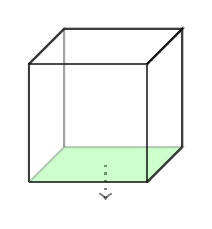
\begin{tikzpicture}[thick,scale=1.5]
    \coordinate (A1) at (0, 0);
    \coordinate (A2) at (0, 1);
    \coordinate (A3) at (1, 1);
    \coordinate (A4) at (1, 0);
    \coordinate (B1) at (0.3, 0.3);
    \coordinate (B2) at (0.3, 1.3);
    \coordinate (B3) at (1.3, 1.3);
    \coordinate (B4) at (1.3, 0.3);
    \coordinate (R1) at (0.65, 0.15);
    \coordinate (R2) at (0.65, -0.15);

	\draw[->, dotted, opacity=0.5] (R1) -- (R2);
	
%1 green
%2 violet
%3 red
%4 orange
%5 yellow
%6 pink

    \draw[fill=green, opacity=0.2] (A1) -- (B1) -- (B4) -- (A4); % bottom
    \draw[opacity=0.2] (A1) -- (A2) -- (B2) -- (B1); % left
    \draw[opacity=0.2] (B1) -- (B2) -- (B3) -- (B4); % back
    \draw[opacity=0.7] (A3) -- (B3) -- (B4) -- (A4); % right
    \draw[opacity=0.7] (A2) -- (B2) -- (B3) -- (A3); % top
    \draw[opacity=0.7] (A1) -- (A2) -- (A3) -- (A4) -- (A1) -- (A1); % front
    
\end{tikzpicture}
\caption{6 possible locations that each face can occupy ($|\operatorname{orb}_{C}(f)| = 6$)}
\label{orb}
\end{figure}

Equipped with these definitions, we can now consider the \emph{Orbit-Stabilizer Theorem}.  This theorem is a counting theorem that allows us to find the number of elements in a permutation group.  The theorem is stated by Gallian as follows:
\begin{quote}
Let $G$ be a finite group of permutations of a set $S$.  Then, for any $i$ from $S$, $|G| = |\operatorname{orb}_G(i)|\,|\operatorname{stab}_G(i)|$. (Gallian 152)
\end{quote}

Using the concept of cosets and Lagrange's Theorem, the Orbit-Stabilizer Theorem can be proven.  To use Lagrange's Theorem, we must first convince ourselves that $\operatorname{stab}_G(i)$ is a subgroup of $G$.
\begin{proof}
Suppose $\psi, \phi \in \operatorname{stab}_G(i)$.  Then $(\psi \circ \phi)(i) = (\psi \circ (\phi(i)) =  (\psi)(i) = i$, so $\operatorname{stab}_G(i)$ is closed under composition.  Since $\phi(i) = i$, the identity certainly exists.  Lastly, $\phi(i) = i$ implies that $\phi^{-1}(\phi(i)) = \phi^{-1}(i)$.   So $\phi^{-1}(i) = i$, which means an inverse exists for all $i\in \operatorname{stab}_G(i)$.
\end{proof}
Lagrange's Theorem then allows us to assert that $|G|/|\operatorname{stab}_G(i)|$ is the number of distinct left cosets of $\operatorname{stab}_G(i)$ in $G$.  For the proof, Gallian maps a coset to elements in the orbit of $i$ and proves that the mapping is a well-defined function, and that the function is a bijection. (Gallian 152)

According the Orbit-Stabilizer Theorem, the cube should have $|\operatorname{stab}_{C}(f)|\, |\operatorname{orb}_{C}(f)| = 4 \cdot 6 = 24$ rotational symmetries, while the tetrahedron should have $|\operatorname{stab}_{T}(f)|\, |\operatorname{orb}_{T}(f)| = 3 \cdot 4 = 12$ rotational symmetries.  To verify these results, let us explore both polyhedra.  First consider the cube.  As stated before, a particular face can occupy $6$ different locations -- I will number them $\{ 1,2,3,4,5,6 \}$ ($\operatorname{orb}_{C}(f)$).  Each location can be rotated in the following ways: $\{ R_0, R_{90}, R_{180}, R_{270} \}$ ($\operatorname{stab}_{C}(f)$).  A similar scheme can be used for a tetrahedron ($\operatorname{orb}_{T}(f) = \{ 1,2,3,4 \}$, and $\operatorname{stab}_{T}(f) = \{ R_0, R_{120}, R_{240} \}$).  When listed out in Table \ref{symcube} and \ref{symtet}, we find that the theorem holds true.
\begin{table}[H]
    \begin{minipage}{.5\linewidth}
\centering
\begin{tabular}{| c | c | c | c | c | c |}
\hline
$1_{R_{0}}$     &  $2_{R_{0}}$     &  $3_{R_{0}}$     &  $4_{R_{0}}$     &  $5_{R_{0}}$     &  $6_{R_{0}}$  \\
$1_{R_{90}}$   &  $2_{R_{90}}$   &  $3_{R_{90}}$   &  $4_{R_{90}}$   &  $5_{R_{90}}$    &  $6_{R_{90}}$  \\
$1_{R_{180}}$ &  $2_{R_{180}}$ &  $3_{R_{180}}$  &  $4_{R_{180}}$ &  $5_{R_{180}}$  &  $6_{R_{180}}$ \\
$1_{R_{270}}$ &  $2_{R_{270}}$ &  $3_{R_{270}}$  &  $4_{R_{270}}$ &  $5_{R_{270}}$  &  $6_{R_{270}}$  \\\hline
\end{tabular}\vspace{2mm}
\caption{Symmetries of a Cube}
\label{symcube}
\end{minipage}%
\begin{minipage}{.5\linewidth}
\centering
\begin{tabular}{| c | c | c | c | c | c |}
\hline
$1_{R_{0}}$     &  $2_{R_{0}}$     &  $3_{R_{0}}$     &  $4_{R_{0}}$  \\
$1_{R_{120}}$   &  $2_{R_{120}}$   &  $3_{R_{120}}$   &  $4_{R_{120}}$  \\
$1_{R_{240}}$ &  $2_{R_{240}}$ &  $3_{R_{240}}$  &  $4_{R_{240}}$  \\\hline
\end{tabular}\vspace{2mm}
\caption{Symmetries of a Tetrahedron}
\label{symtet}
\end{minipage}
\end{table}
Taking these concepts further, we can explore the properties of more shapes.  Another example we can look at is the octahedron.  Having $8$ faces, any particular face can occupy any of $8$ locations, which represents the orbit of that element in the group.  Rotating about the center of a fixed face, the octahedron has $3$ possible positions, which represents the stabilizer of the element in the group.  Once more, by using the Orbit-Stabilizer Theorem, we find that the total rotational symmetries of the octahedron is $24$.  Similarly, the dodecahedron can be examined.  Let $D = \{ \text{rotational symmetries of a dodecahedron} \}$.  Then this $12$ sided polyhedron ($|\operatorname{orb}_{D}(f)| = 12$) with pentagonal sides ($|\operatorname{stab}_{D}(f)| = 5$) has $|D| = |\operatorname{orb}_{D}(f)|\,|\operatorname{stab}_{D}(f)| = 60$ rotational symmetries.

If you observe carefully, we are not limited to using faces for the orbit or stabilizer for a polyhedron.  In fact, it is by manipulating the orbit and stabilizer of a cube that Gallian proves another theorem that states "the group of rotations of a cube is isomorphic to $S_4$." (Gallian 154)  By using a diagonal of the cube for the orbit and stabilizer, we can construct an isomorphism to $S_4$.  Let $D = \{ \text{diagonals of a cube} \}$ and $d \in D$.  If we rotate the cube 90 degrees about the "y-axis" (call this operation $\alpha = (1234)$) and/or the "x-axis" ($\beta = (1423)$), we can create an eight element subgroup $\operatorname{orb}_{C}(d) = \{ \varepsilon, \alpha, \alpha^2, \alpha^3, \beta^2, \beta^2\alpha, \beta^2\alpha^2, \beta^2\alpha^3  \}$ (Figure \ref{oS4}).  Furthermore, by fixing $d$, we can produce three permutations by executing the $\alpha\beta$ operation, which has an order of $3$ (Figure \ref{sS4}).  Together, the rotations produce all $24$ rotational symmetries of a cube as well as all permutations of $S_4$.
\begin{figure}[H]\centering
 \begin{minipage}{.2\linewidth}\centering
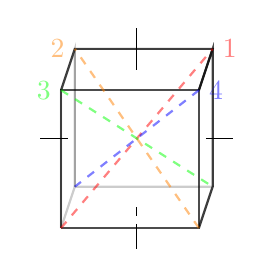
\begin{tikzpicture}[thick, scale=1.75]
    \coordinate (A1) at (0, 0);
    \coordinate (A2) at (0, 1);
    \coordinate (A3) at (1, 1);
    \coordinate (A4) at (1, 0);
    \coordinate (B1) at (0.1, 0.3);
    \coordinate (B2) at (0.1, 1.3);
    \coordinate (B3) at (1.1, 1.3);
    \coordinate (B4) at (1.1, 0.3);
	
%1 green
%2 violet
%3 red
%4 orange
%5 yellow
%6 pink

    \draw[opacity=0.2] (A1) -- (B1) -- (B4) -- (A4); % bottom
    \draw[opacity=0.2] (A1) -- (A2) -- (B2) -- (B1); % left
    \draw[opacity=0.2] (B1) -- (B2) -- (B3) -- (B4); % back
    \draw[opacity=0.7] (A3) -- (B3) -- (B4) -- (A4); % right
    \draw[opacity=0.7] (A2) -- (B2) -- (B3) -- (A3); % top
    \draw[opacity=0.7] (A1) -- (A2) -- (A3) -- (A4) -- (A1) -- (A1); % front

	\draw[red, opacity=0.5, dashed] (A1) -- (B3) node[anchor=west]{1} ; % 1
	\draw[orange, opacity=0.5, dashed] (A4) -- (B2) node[anchor=east]{2}; % 2
    \draw[green, opacity=0.5, dashed] (A2) node[anchor=east]{3} -- (B4); % 3
    \draw[blue, opacity=0.5, dashed] (A3) node[anchor=west]{4} -- (B1); % 4
    
    \draw[thin, solid] (0.55, 1.15) -- (0.55, 1.45); 
    \draw[thin, dashed] (0.55, 0.15) -- (0.55, 0);
    \draw[thin, solid] (0.55, 0) -- (0.55, -0.15);  
    
    \draw[thin, solid] (1.05, 0.65) -- (1.25, 0.65); 
    \draw[thin, dashed] (0.05, 0.65) -- (0, 0.65);
    \draw[thin, solid] (-0.15, 0.65) -- (0, 0.65);  
    
\end{tikzpicture}
\captionsetup{labelformat=empty}
\caption*{$\varepsilon$}
\end{minipage}
 \begin{minipage}{.2\linewidth}\centering
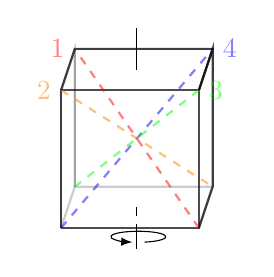
\begin{tikzpicture}[thick, scale=1.75]
    \coordinate (A1) at (0, 0);
    \coordinate (A2) at (0, 1);
    \coordinate (A3) at (1, 1);
    \coordinate (A4) at (1, 0);
    \coordinate (B1) at (0.1, 0.3);
    \coordinate (B2) at (0.1, 1.3);
    \coordinate (B3) at (1.1, 1.3);
    \coordinate (B4) at (1.1, 0.3);
	
%1 green
%2 violet
%3 red
%4 orange
%5 yellow
%6 pink

    \draw[opacity=0.2] (A1) -- (B1) -- (B4) -- (A4); % bottom
    \draw[opacity=0.2] (A1) -- (A2) -- (B2) -- (B1); % left
    \draw[opacity=0.2] (B1) -- (B2) -- (B3) -- (B4); % back
    \draw[opacity=0.7] (A3) -- (B3) -- (B4) -- (A4); % right
    \draw[opacity=0.7] (A2) -- (B2) -- (B3) -- (A3); % top
    \draw[opacity=0.7] (A1) -- (A2) -- (A3) -- (A4) -- (A1) -- (A1); % front

	\draw[blue, opacity=0.5, dashed] (A1) -- (B3) node[anchor=west]{4}; % 4
	\draw[red, opacity=0.5, dashed] (A4) -- (B2) node[anchor=east]{1}; % 1
    \draw[orange, opacity=0.5, dashed] (A2) node[anchor=east]{2} -- (B4); % 2
    \draw[green, opacity=0.5, dashed] (A3) node[anchor=west]{3} -- (B1); % 3
    
    \draw[thin, -latex, xshift=16, yshift=-1.8] (-77.5:2mm and 0.4mm) arc (-77:257.5:2mm and 0.4mm);
    \draw[thin, solid] (0.55, 1.15) -- (0.55, 1.45); 
    \draw[thin, dashed] (0.55, 0.15) -- (0.55, 0);
    \draw[thin, solid] (0.55, 0) -- (0.55, -0.15);  
    
    
\end{tikzpicture}
\captionsetup{labelformat=empty}
\caption*{$\alpha = (1234)$}
\end{minipage}
 \begin{minipage}{.2\linewidth}\centering
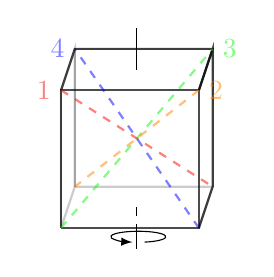
\begin{tikzpicture}[thick, scale=1.75]
    \coordinate (A1) at (0, 0);
    \coordinate (A2) at (0, 1);
    \coordinate (A3) at (1, 1);
    \coordinate (A4) at (1, 0);
    \coordinate (B1) at (0.1, 0.3);
    \coordinate (B2) at (0.1, 1.3);
    \coordinate (B3) at (1.1, 1.3);
    \coordinate (B4) at (1.1, 0.3);
	
%1 green
%2 violet
%3 red
%4 orange
%5 yellow
%6 pink

    \draw[opacity=0.2] (A1) -- (B1) -- (B4) -- (A4); % bottom
    \draw[opacity=0.2] (A1) -- (A2) -- (B2) -- (B1); % left
    \draw[opacity=0.2] (B1) -- (B2) -- (B3) -- (B4); % back
    \draw[opacity=0.7] (A3) -- (B3) -- (B4) -- (A4); % right
    \draw[opacity=0.7] (A2) -- (B2) -- (B3) -- (A3); % top
    \draw[opacity=0.7] (A1) -- (A2) -- (A3) -- (A4) -- (A1) -- (A1); % front

	\draw[green, opacity=0.5, dashed] (A1) -- (B3) node[anchor=west]{3}; %  3
	\draw[blue, opacity=0.5, dashed] (A4) -- (B2) node[anchor=east]{4}; % 4
    \draw[red, opacity=0.5, dashed] (A2) node[anchor=east]{1} -- (B4); % 1
    \draw[orange, opacity=0.5, dashed] (A3) node[anchor=west]{2} -- (B1); % 2
    
    \draw[thin, -latex, xshift=16, yshift=-1.8] (-77.5:2mm and 0.4mm) arc (-77:257.5:2mm and 0.4mm);
    \draw[thin, solid] (0.55, 1.15) -- (0.55, 1.45); 
    \draw[thin, dashed] (0.55, 0.15) -- (0.55, 0);
    \draw[thin, solid] (0.55, 0) -- (0.55, -0.15);  
    
    
\end{tikzpicture}
\captionsetup{labelformat=empty}
\caption*{$\alpha^2 = (13)(24)$}
\end{minipage}
 \begin{minipage}{.2\linewidth}\centering
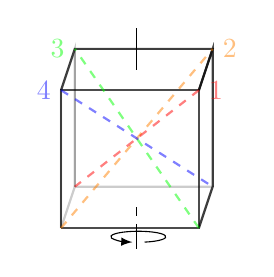
\begin{tikzpicture}[thick, scale=1.75]
    \coordinate (A1) at (0, 0);
    \coordinate (A2) at (0, 1);
    \coordinate (A3) at (1, 1);
    \coordinate (A4) at (1, 0);
    \coordinate (B1) at (0.1, 0.3);
    \coordinate (B2) at (0.1, 1.3);
    \coordinate (B3) at (1.1, 1.3);
    \coordinate (B4) at (1.1, 0.3);
	
%1 green
%2 violet
%3 red
%4 orange
%5 yellow
%6 pink

    \draw[opacity=0.2] (A1) -- (B1) -- (B4) -- (A4); % bottom
    \draw[opacity=0.2] (A1) -- (A2) -- (B2) -- (B1); % left
    \draw[opacity=0.2] (B1) -- (B2) -- (B3) -- (B4); % back
    \draw[opacity=0.7] (A3) -- (B3) -- (B4) -- (A4); % right
    \draw[opacity=0.7] (A2) -- (B2) -- (B3) -- (A3); % top
    \draw[opacity=0.7] (A1) -- (A2) -- (A3) -- (A4) -- (A1) -- (A1); % front

	\draw[orange, opacity=0.5, dashed] (A1) -- (B3) node[anchor=west]{2}; %2
	\draw[green, opacity=0.5, dashed] (A4) -- (B2) node[anchor=east]{3}; % 3
    \draw[blue, opacity=0.5, dashed] (A2) node[anchor=east]{4} -- (B4); % 4
    \draw[red, opacity=0.5, dashed] (A3) node[anchor=west]{1} -- (B1); % 1
    
    \draw[thin, -latex, xshift=16, yshift=-1.8] (-77.5:2mm and 0.4mm) arc (-77:257.5:2mm and 0.4mm);
    \draw[thin, solid] (0.55, 1.15) -- (0.55, 1.45); 
    \draw[thin, dashed] (0.55, 0.15) -- (0.55, 0);
    \draw[thin, solid] (0.55, 0) -- (0.55, -0.15);  
    
    
\end{tikzpicture}
\captionsetup{labelformat=empty}
\caption*{$\alpha^3 = (1432)$}
\end{minipage}\vspace{5mm}
 \begin{minipage}{.2\linewidth}\centering
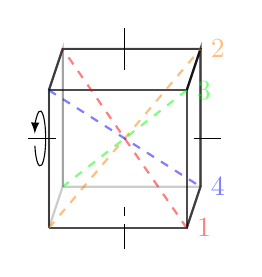
\begin{tikzpicture}[thick, scale=1.75]
    \coordinate (A1) at (0, 0);
    \coordinate (A2) at (0, 1);
    \coordinate (A3) at (1, 1);
    \coordinate (A4) at (1, 0);
    \coordinate (B1) at (0.1, 0.3);
    \coordinate (B2) at (0.1, 1.3);
    \coordinate (B3) at (1.1, 1.3);
    \coordinate (B4) at (1.1, 0.3);
	
%1 green
%2 violet
%3 red
%4 orange
%5 yellow
%6 pink

    \draw[opacity=0.2] (A1) -- (B1) -- (B4) -- (A4); % bottom
    \draw[opacity=0.2] (A1) -- (A2) -- (B2) -- (B1); % left
    \draw[opacity=0.2] (B1) -- (B2) -- (B3) -- (B4); % back
    \draw[opacity=0.7] (A3) -- (B3) -- (B4) -- (A4); % right
    \draw[opacity=0.7] (A2) -- (B2) -- (B3) -- (A3); % top
    \draw[opacity=0.7] (A1) -- (A2) -- (A3) -- (A4) -- (A1) -- (A1); % front

	\draw[orange, opacity=0.5, dashed] (A1) -- (B3) node[anchor=west]{2}; % 4
	\draw[red, opacity=0.5, dashed] (A4) node[anchor=west]{1} -- (B2); % 1
    \draw[blue, opacity=0.5, dashed] (A2)-- (B4) node[anchor=west]{4} ; % 2
    \draw[green, opacity=0.5, dashed] (A3) node[anchor=west]{3} -- (B1); % 3
    
    \draw[thin, -latex, yshift=18.5, xshift=-1.8] (-165:0.4mm and 2mm) arc (-165:170:0.4mm and 2mm);
    \draw[thin, solid] (1.05, 0.65) -- (1.25, 0.65); 
    \draw[thin, dashed] (0.05, 0.65) -- (0, 0.65);
    \draw[thin, solid] (-0.15, 0.65) -- (0, 0.65);  
    \draw[thin, solid] (0.55, 1.15) -- (0.55, 1.45); 
    \draw[thin, dashed] (0.55, 0.15) -- (0.55, 0);
    \draw[thin, solid] (0.55, 0) -- (0.55, -0.15);  
    
    
\end{tikzpicture}
\captionsetup{labelformat=empty}
\caption*{$\beta^2 = (12)(34)$}
\end{minipage}
 \begin{minipage}{.2\linewidth}\centering
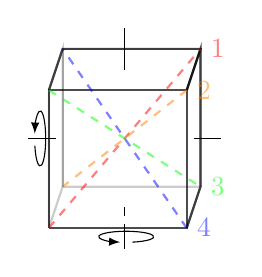
\begin{tikzpicture}[thick, scale=1.75]
    \coordinate (A1) at (0, 0);
    \coordinate (A2) at (0, 1);
    \coordinate (A3) at (1, 1);
    \coordinate (A4) at (1, 0);
    \coordinate (B1) at (0.1, 0.3);
    \coordinate (B2) at (0.1, 1.3);
    \coordinate (B3) at (1.1, 1.3);
    \coordinate (B4) at (1.1, 0.3);
	
%1 green
%2 violet
%3 red
%4 orange
%5 yellow
%6 pink

    \draw[opacity=0.2] (A1) -- (B1) -- (B4) -- (A4); % bottom
    \draw[opacity=0.2] (A1) -- (A2) -- (B2) -- (B1); % left
    \draw[opacity=0.2] (B1) -- (B2) -- (B3) -- (B4); % back
    \draw[opacity=0.7] (A3) -- (B3) -- (B4) -- (A4); % right
    \draw[opacity=0.7] (A2) -- (B2) -- (B3) -- (A3); % top
    \draw[opacity=0.7] (A1) -- (A2) -- (A3) -- (A4) -- (A1) -- (A1); % front

	\draw[red, opacity=0.5, dashed] (A1) -- (B3) node[anchor=west]{1}; % 1
	\draw[blue, opacity=0.5, dashed] (A4) node[anchor=west]{4} -- (B2); % 2
    \draw[green, opacity=0.5, dashed] (A2) -- (B4) node[anchor=west]{3}; % 3
    \draw[orange, opacity=0.5, dashed] (A3) node[anchor=west]{2} -- (B1); % 4
    
    \draw[thin, -latex, yshift=18.5, xshift=-1.8] (-165:0.4mm and 2mm) arc (-165:170:0.4mm and 2mm);
    \draw[thin, solid] (1.05, 0.65) -- (1.25, 0.65); 
    \draw[thin, dashed] (0.05, 0.65) -- (0, 0.65);
    \draw[thin, solid] (-0.15, 0.65) -- (0, 0.65);  
    
    \draw[thin, -latex, xshift=16, yshift=-1.8] (-77.5:2mm and 0.4mm) arc (-77:257.5:2mm and 0.4mm);
    \draw[thin, solid] (0.55, 1.15) -- (0.55, 1.45); 
    \draw[thin, dashed] (0.55, 0.15) -- (0.55, 0);
    \draw[thin, solid] (0.55, 0) -- (0.55, -0.15);  
    
    
\end{tikzpicture}
\captionsetup{labelformat=empty}
\caption*{$\beta^2\alpha = (24)$}
\end{minipage}
 \begin{minipage}{.2\linewidth}\centering
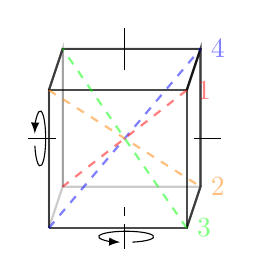
\begin{tikzpicture}[thick, scale=1.75]
    \coordinate (A1) at (0, 0);
    \coordinate (A2) at (0, 1);
    \coordinate (A3) at (1, 1);
    \coordinate (A4) at (1, 0);
    \coordinate (B1) at (0.1, 0.3);
    \coordinate (B2) at (0.1, 1.3);
    \coordinate (B3) at (1.1, 1.3);
    \coordinate (B4) at (1.1, 0.3);
	
%1 green
%2 violet
%3 red
%4 orange
%5 yellow
%6 pink

    \draw[opacity=0.2] (A1) -- (B1) -- (B4) -- (A4); % bottom
    \draw[opacity=0.2] (A1) -- (A2) -- (B2) -- (B1); % left
    \draw[opacity=0.2] (B1) -- (B2) -- (B3) -- (B4); % back
    \draw[opacity=0.7] (A3) -- (B3) -- (B4) -- (A4); % right
    \draw[opacity=0.7] (A2) -- (B2) -- (B3) -- (A3); % top
    \draw[opacity=0.7] (A1) -- (A2) -- (A3) -- (A4) -- (A1) -- (A1); % front

	\draw[blue, opacity=0.5, dashed] (A1) -- (B3) node[anchor=west]{4}; %2
	\draw[green, opacity=0.5, dashed] (A4) node[anchor=west]{3} -- (B2); % 3
    \draw[orange, opacity=0.5, dashed] (A2) -- (B4) node[anchor=west]{2}; % 4
    \draw[red, opacity=0.5, dashed] (A3) node[anchor=west]{1} -- (B1); % 1
    
    \draw[thin, -latex, yshift=18.5, xshift=-1.8] (-165:0.4mm and 2mm) arc (-165:170:0.4mm and 2mm);
    \draw[thin, solid] (1.05, 0.65) -- (1.25, 0.65); 
    \draw[thin, dashed] (0.05, 0.65) -- (0, 0.65);
    \draw[thin, solid] (-0.15, 0.65) -- (0, 0.65);  
    
    \draw[thin, -latex, xshift=16, yshift=-1.8] (-77.5:2mm and 0.4mm) arc (-77:257.5:2mm and 0.4mm);
    \draw[thin, solid] (0.55, 1.15) -- (0.55, 1.45); 
    \draw[thin, dashed] (0.55, 0.15) -- (0.55, 0);
    \draw[thin, solid] (0.55, 0) -- (0.55, -0.15);  
    
    
\end{tikzpicture}
\captionsetup{labelformat=empty}
\caption*{$\beta^2\alpha^2 = (14)(23)$}
\end{minipage}
 \begin{minipage}{.2\linewidth}\centering
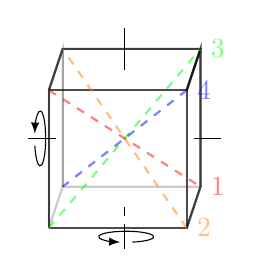
\begin{tikzpicture}[thick, scale=1.75]
    \coordinate (A1) at (0, 0);
    \coordinate (A2) at (0, 1);
    \coordinate (A3) at (1, 1);
    \coordinate (A4) at (1, 0);
    \coordinate (B1) at (0.1, 0.3);
    \coordinate (B2) at (0.1, 1.3);
    \coordinate (B3) at (1.1, 1.3);
    \coordinate (B4) at (1.1, 0.3);
	
%1 green
%2 violet
%3 red
%4 orange
%5 yellow
%6 pink

    \draw[opacity=0.2] (A1) -- (B1) -- (B4) -- (A4); % bottom
    \draw[opacity=0.2] (A1) -- (A2) -- (B2) -- (B1); % left
    \draw[opacity=0.2] (B1) -- (B2) -- (B3) -- (B4); % back
    \draw[opacity=0.7] (A3) -- (B3) -- (B4) -- (A4); % right
    \draw[opacity=0.7] (A2) -- (B2) -- (B3) -- (A3); % top
    \draw[opacity=0.7] (A1) -- (A2) -- (A3) -- (A4) -- (A1) -- (A1); % front

	\draw[green, opacity=0.5, dashed] (A1) -- (B3) node[anchor=west]{3}; %  3
	\draw[orange, opacity=0.5, dashed] (A4) node[anchor=west]{2} -- (B2); % 4
    \draw[red, opacity=0.5, dashed] (A2) -- (B4) node[anchor=west]{1}; % 1
    \draw[blue, opacity=0.5, dashed] (A3) node[anchor=west]{4} -- (B1); % 2
    
    \draw[thin, -latex, yshift=18.5, xshift=-1.8] (-165:0.4mm and 2mm) arc (-165:170:0.4mm and 2mm);
    \draw[thin, solid] (1.05, 0.65) -- (1.25, 0.65); 
    \draw[thin, dashed] (0.05, 0.65) -- (0, 0.65);
    \draw[thin, solid] (-0.15, 0.65) -- (0, 0.65);  
    
    \draw[thin, -latex, xshift=16, yshift=-1.8] (-77.5:2mm and 0.4mm) arc (-77:257.5:2mm and 0.4mm);
    \draw[thin, solid] (0.55, 1.15) -- (0.55, 1.45); 
    \draw[thin, dashed] (0.55, 0.15) -- (0.55, 0);
    \draw[thin, solid] (0.55, 0) -- (0.55, -0.15);  
    
    
\end{tikzpicture}
\captionsetup{labelformat=empty}
\caption*{$\beta^2\alpha^3 = (13)$}
\end{minipage}
\caption{8 possible locations that the diagonals can occupy ($|\operatorname{orb}_{C}(d)| = 8$)}
\label{oS4}
\end{figure}
%%%%%%%%%%%%%% ALPHA BETA  %%%%%%%%%%%%%%%%%%%%%%%
\begin{figure}[H]
\centering
 \begin{minipage}{.3\linewidth}
\centering
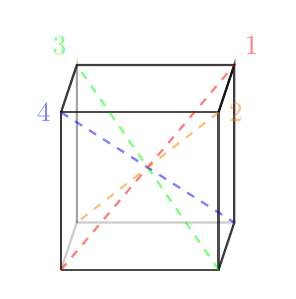
\begin{tikzpicture}[thick,scale=2]
    \coordinate (A1) at (0, 0);
    \coordinate (A2) at (0, 1);
    \coordinate (A3) at (1, 1);
    \coordinate (A4) at (1, 0);
    \coordinate (B1) at (0.1, 0.3);
    \coordinate (B2) at (0.1, 1.3);
    \coordinate (B3) at (1.1, 1.3);
    \coordinate (B4) at (1.1, 0.3);
	
%1 green
%2 violet
%3 red
%4 orange
%5 yellow
%6 pink

    \draw[opacity=0.2] (A1) -- (B1) -- (B4) -- (A4); % bottom
    \draw[opacity=0.2] (A1) -- (A2) -- (B2) -- (B1); % left
    \draw[opacity=0.2] (B1) -- (B2) -- (B3) -- (B4); % back
    \draw[opacity=0.7] (A3) -- (B3) -- (B4) -- (A4); % right
    \draw[opacity=0.7] (A2) -- (B2) -- (B3) -- (A3); % top
    \draw[opacity=0.7] (A1) -- (A2) -- (A3) -- (A4) -- (A1) -- (A1); % front

	\draw[red, opacity=0.5, dashed] (A1) -- (B3) node[anchor=south west]{1}; % 4
	\draw[green, opacity=0.5, dashed] (A4) -- (B2) node[anchor=south east]{3}; % 1
    \draw[blue, opacity=0.5, dashed] (A2) node[anchor=east]{4} -- (B4); % 2
    \draw[orange, opacity=0.5, dashed] (A3) node[anchor=west]{2} -- (B1); % 3
    
    
\end{tikzpicture}
\captionsetup{labelformat=empty}
\caption*{$\alpha\beta = (243)$}
\end{minipage}
 \begin{minipage}{.3\linewidth}
\centering
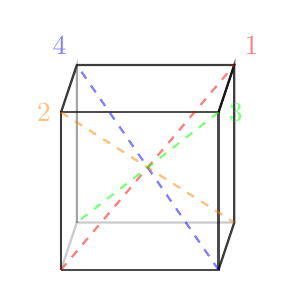
\begin{tikzpicture}[thick,scale=2]
    \coordinate (A1) at (0, 0);
    \coordinate (A2) at (0, 1);
    \coordinate (A3) at (1, 1);
    \coordinate (A4) at (1, 0);
    \coordinate (B1) at (0.1, 0.3);
    \coordinate (B2) at (0.1, 1.3);
    \coordinate (B3) at (1.1, 1.3);
    \coordinate (B4) at (1.1, 0.3);
	
%1 green
%2 violet
%3 red
%4 orange
%5 yellow
%6 pink

    \draw[opacity=0.2] (A1) -- (B1) -- (B4) -- (A4); % bottom
    \draw[opacity=0.2] (A1) -- (A2) -- (B2) -- (B1); % left
    \draw[opacity=0.2] (B1) -- (B2) -- (B3) -- (B4); % back
    \draw[opacity=0.7] (A3) -- (B3) -- (B4) -- (A4); % right
    \draw[opacity=0.7] (A2) -- (B2) -- (B3) -- (A3); % top
    \draw[opacity=0.7] (A1) -- (A2) -- (A3) -- (A4) -- (A1) -- (A1); % front

	\draw[red, opacity=0.5, dashed] (A1) -- (B3) node[anchor=south west]{1}; %  3
	\draw[blue, opacity=0.5, dashed] (A4) -- (B2) node[anchor=south east]{4}; % 4
    \draw[orange, opacity=0.5, dashed] (A2) node[anchor=east]{2} -- (B4); % 1
    \draw[green, opacity=0.5, dashed] (A3) node[anchor=west]{3} -- (B1); % 2
    
    
\end{tikzpicture}
\captionsetup{labelformat=empty}
\caption*{$(\alpha\beta)^2 = (234)$}
\end{minipage}
 \begin{minipage}{.3\linewidth}
\centering
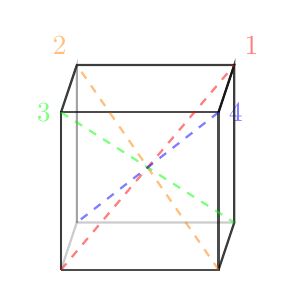
\begin{tikzpicture}[thick,scale=2]
    \coordinate (A1) at (0, 0);
    \coordinate (A2) at (0, 1);
    \coordinate (A3) at (1, 1);
    \coordinate (A4) at (1, 0);
    \coordinate (B1) at (0.1, 0.3);
    \coordinate (B2) at (0.1, 1.3);
    \coordinate (B3) at (1.1, 1.3);
    \coordinate (B4) at (1.1, 0.3);
	
%1 green
%2 violet
%3 red
%4 orange
%5 yellow
%6 pink

    \draw[opacity=0.2] (A1) -- (B1) -- (B4) -- (A4); % bottom
    \draw[opacity=0.2] (A1) -- (A2) -- (B2) -- (B1); % left
    \draw[opacity=0.2] (B1) -- (B2) -- (B3) -- (B4); % back
    \draw[opacity=0.7] (A3) -- (B3) -- (B4) -- (A4); % right
    \draw[opacity=0.7] (A2) -- (B2) -- (B3) -- (A3); % top
    \draw[opacity=0.7] (A1) -- (A2) -- (A3) -- (A4) -- (A1) -- (A1); % front

	\draw[red, opacity=0.5, dashed] (A1) -- (B3) node[anchor=south west]{1} ; % 1
	\draw[orange, opacity=0.5, dashed] (A4) -- (B2) node[anchor=south east]{2}; % 2
    \draw[green, opacity=0.5, dashed] (A2) node[anchor=east]{3} -- (B4); % 3
    \draw[blue, opacity=0.5, dashed] (A3) node[anchor=west]{4} -- (B1); % 4
    
\end{tikzpicture}
\captionsetup{labelformat=empty}
\caption*{$(\alpha\beta)^3 = \varepsilon$}
\end{minipage}
\caption{3 possible permutations with diagonal $1$ fixed ($|\operatorname{stab}_{C}(d)| = 3$)}
\label{sS4}
\end{figure}

To conclude, I leave you with a final example of a shape that more complicated than those explored earlier.  The truncated icosahedron is the shape of a soccer ball with $32$ faces, and the faces come in two types: $20$ regular hexagons and $12$ regular pentagons.  Despite this, the shape can still be analyzed with the Orbit-Stabilizer Theorem.  If we choose our set to be the set of $12$ pentagons, each pantagon can be carried to any of the other pentagons through some sort of rotation. This means that the size of the orbit of any pentagon is $12$.  Additionally, fixing any pentagon, we can rotate the object $72$ degrees while maintaining symmetry, and this rotation has an order of $5$.  So, by the Orbit-Stabilizer Theorem, this shape has $60$ rotational symmetries.  If we choose the hexagons for our set, we find that $|\operatorname{orb}_{H}(f)| = 20$.  Something of note with the stabilizer is that although a hexagon has $6$ sides, the object can only maintain symmetry when it is rotated $120$ degrees, so $|\operatorname{stab}_{H}(f)| = 3$.  Once again, this matches our earlier finding of the number of rotational symmetries of this shape.

\end{document}
